\chapter{Аналитическая часть}

\section{Трассировка лучей}

\subsection{Классическая трассировка лучей}

%Классический метод трассировки лучей реализует отслеживание траекторий лучей и расчета взаимодействий с лежащими на траекториях объектами, от момента испускания лучей источником света до момента попадания в камеру.
 
%Под взаимодействием луча с объектами понимаются процессы диффузного, многократного зеркального отражения от их поверхности и прохождения лучей сквозь прозрачные объекты.

%Трассировка лучей -- первый метод расчета глобального освещения, рассматривающий освещение, затенение, многократные отражения и преломления. Различают два подхода к трассировке лучей: метод прямой трассировки и метод обратной трассировки. В классической трассировке лучей лучи света обрабатываются в обратном направлении: луч испускается из камеры вглубь сцены через пиксель окна вывода.

Трассировка лучей (англ. ray tracing) -- метод синтеза компьютерных изображений, который позволяет добиться повышения качества синтезируемого изображения за счёт повышения затрат вычислительных ресурсов.
Для каждого пикселя в итоговом изображении математический луч проецируется в трехмерном пространстве из камеры через пиксель по направлению к сцене. В классическом варианте луч сталкивается с объектом сцены, и, не учитывая отражение и прозрачность, с помощью цвета объекта, определяется цвет соответствующего пикселя в синтезируемом изображении. На рисунке \ref{img:ray-tracing} представлено схематическое представление построения изображения методом трассировки лучей.

\begin{figure}[H]
	\begin{center}
		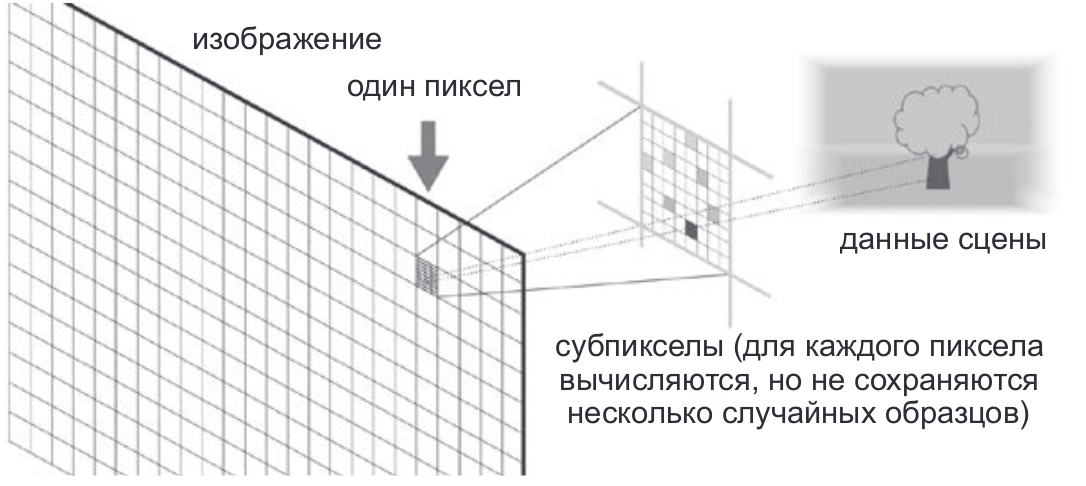
\includegraphics[scale=0.4]{img/ray_tracing.png}
	\end{center}
	\captionsetup{justification=centering}
	\caption{Представление построения изображения методом трассировки лучей.}
	\label{img:ray-tracing}
\end{figure}


Хотя при отслеживании всего одного луча на пиксель будет построено правильное изображение, удаленные подробности (такие как дерево на рисунке \ref{img:ray-tracing}) сцены будут потеряны. Кроме того, при перемещении камеры объекта могут появляться шумовые эффекты \cite{what-is-noise}. Ни рисунке \ref{img:noise-example} представленно изображение с шумовыми эффектами.

\begin{figure}[H]
	\begin{center}
		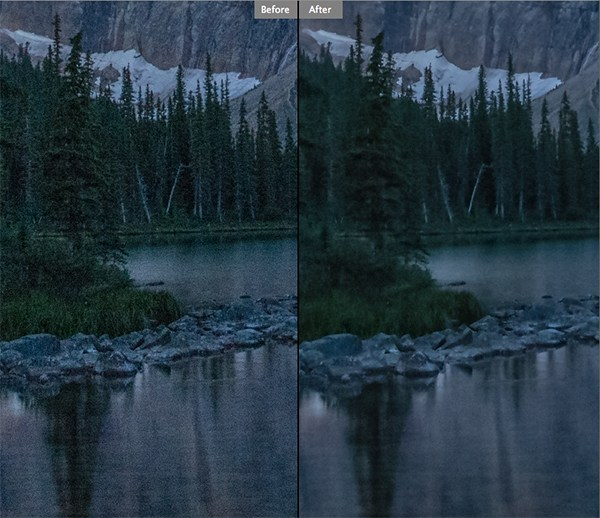
\includegraphics[scale=0.8]{img/noise-example.jpg}
	\end{center}
	\captionsetup{justification=centering}
	\caption{Слева -- изображение с шумовыми эффектами, справа -- тоже самое изображение без шумовых эффектов.}
	\label{img:noise-example}
\end{figure}


\subsection{Трассировка лучей методом Монте-Карло}

Для того чтобы решить задачу без увеличения размеров изображения, программы трассировки лучей проецируют несколько лучей на пиксель, с небольшим изменением направлением для каждого луча. В таком случае, сохраняется только среднее значение цвета, а остальные значения не используются. На рисунке \ref{img:ray-tracing} схематично изображена проекция нескольких лучей на один пиксель.

 Процес получения одного среднего значения называют избыточной выборкой (англ. supersamling), или выборкой по методу Монте-Карло. Трассировку лучей с использованием такого алгоритма называют трассировкой лучей методом Монте-Карло. Чем больше образцов (англ. sample) будет получено, тем ниже будет уровень шума в итоговом изображении. Избыточная выборка -- важный шаг в процессе обработки изображений, синтезированных компьютером.

В избыточной выборке возможна параллельная обработка -- подсчет результатов проекции множества лучей на сцену, данную задачу очень легко распараллелить. Но, в конечном итоге используются не отдельные результаты, а только их среднее значение. 

Избыточная выборка является задачей где можно эффективно применить квантовые вычисления \cite{PQC-classic}. Это становится возможным, потому что квантовые вычисления обладают свойством квантовой суперпозиции \cite{qsp} и принципом квантовой запутанности \cite{qtheory}.

\section{Квантовая обработка изображений}

Технология квантовой обработки изображений использует квантовые вычисления для расширения возможностей обработки и синтеза изображений. Данная технология находится на начальной стадии развития \cite{state}, в связи с этим на нас наложен ряд ограничений. Во-первых, в настоящий момент, квантовые компьютеры не доступны для широкого использования. Из-за этого, все квантовые вычисления мы можем только лишь эмулировать. Во-вторых, для эмуляции квантовых вычислений нужно большое количество оперативной памяти, размер которой растет экспоненциально \cite{emulating}. В связи с этим мы ограниченны вычислительными мощностями современных компьютеров.

\subsection{Использование избыточной выборки}

Одним из применений квантовых вычислений, которое подходит под условие поставленной задачи, является квантовая избыточная выборка (англ. quantum supersampling). Метод квантовой избыточной выборки в итоге получает результат примерно такой же, как и у существующего классического аналога \cite{PQC-classic}. Но, изображение полученное квантовой выборкой обладает другими преимуществами: средний уровень шума в изображениях, полученных в результате традиционной выборки примерно одинаков, но характер шума сильно различается \cite{PQC-classic}. В изображениях с квантовой выборкой некоторые пиксели сильно зашумлены, тогда как цвет остальных определен без каких-либо ошибок вообще.
 
Таким образом, квантовая выборка выигрывает у традиционной при необходимости пост-обработки синтезируемого изображения, например, удаления всего видимого шума. В случае квантовой выборки этот процес относительно прост, так как на полученном изображении будут пиксели изображенные без каких-либо ошибок либо сильно выделяющиеся пиксели. Сравнение выборок приведено на рисунке \ref{img:compare}.
 
\begin{figure}[H]
 	\begin{center}
 		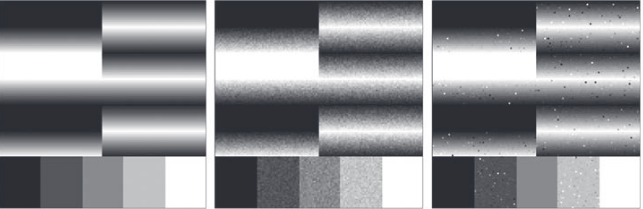
\includegraphics[scale=0.7]{img/compare.png}
 	\end{center}
 	\captionsetup{justification=centering}
 	\caption{Изменение характера шума. Первое изображение -- эталонное; второе -- выборка по методу Монте-Карло; третье -- квантовая выборка.}
 	\label{img:compare}
\end{figure}

К сожалению, для реализации полноценного квантового трассировщика лучей, потребуется намного больше квантовых мощностей, чем доступно в данный момент \cite{PQC-limits}. Из-за этого, в данной работе возможно реализовать только метод квантовой избыточной выборки в качестве той части алгоритма, которую возможно заменить на квантовую.

\section{Основные положения квантовых вычислений}

\subsection{Квантовый бит}

В квантовых вычислениях физические свойства квантовых объектов реализованы в кубитах (англ. quantum bit). Классический бит принимает только два значения – 0 или 1. Кубит до измерения принимает одновременно оба значения. Из-за этого, кубит принято обозначать выражением $a\ket{0}$ + $b\ket{1}$, где $\alpha$ и $\beta$ — комплексные числа, удовлетворяющие условию (\ref{for:ver})

\begin{equation}
\label{for:ver}
|\alpha|^2 + |\beta|^2 = 1. 
\end{equation} 

Измерение кубита мгновенно «схлопывает»  его состояние в базисное – 0 или 1. Вероятности перехода в эти состояние равны соотвественно $|\alpha|^2$ и $|\beta|^2$. 

На рисунке \ref{img:qbits_table} представлена возможная интерпретация состояния кубита в графической форме. Возможные состояния кубита представленны в виде кругов, серое наполнение -- вероятность нахождения кубита в данном состоянии.

\begin{figure}[H]
	\begin{center}
		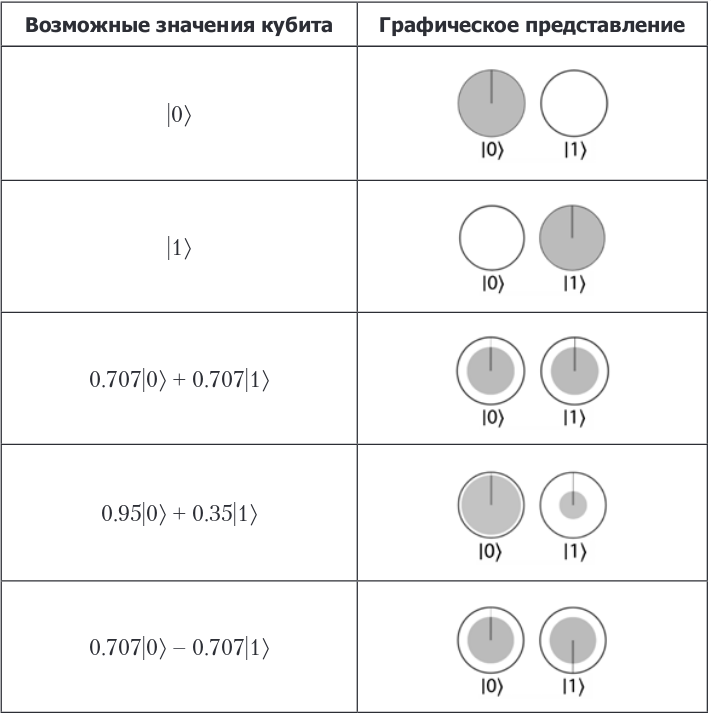
\includegraphics[scale=0.45]{img/qbits.png}
	\end{center}
	\captionsetup{justification=centering}
	\caption{Возможные значения кубита и их представление.}
	\label{img:qbits_table}
\end{figure}

\subsection{Квантовый регистр}

На кубиты может быть наложена ненаблюдаемая связь -- при всяком изменении над одним из нескольких кубитов остальные меняются согласованно с ним. Таким образом, можно интерпретировать такую совокупность кубитов как квантовый регистр. Такой регистр может находиться во всех комбинациях составляющих его битов, и, кроме этого, реализовывать зависимости между ними.

На рис \ref{img:qint} показано одно из возможных представлений квантовых регистров. Это представление использует введенное нами представление кубитов в виде кругов из рисунка \ref{img:qbits_table}.

\begin{figure}[H]
	\begin{center}
		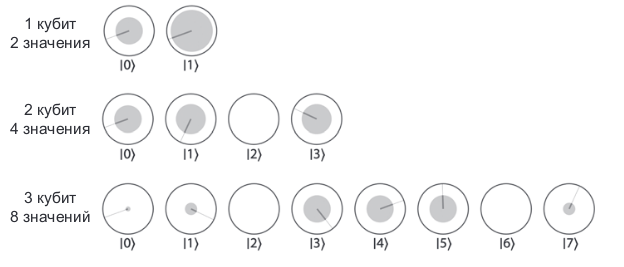
\includegraphics[scale=0.7]{img/qint.png}
	\end{center}
	\captionsetup{justification=centering}
	\caption{Графическое представление квантового регистра.}
	\label{img:qint}
\end{figure}

Согласно принципу суперпозиции квантовый регистр из $n$ кубитов может находиться и во многих других состояниях, которые описываются волновыми функциями, являющимися линейными комбинациями базисных волновых функций (\ref{for:qint}): 

\begin{equation} 
	\label{for:qint}
	\Psi = \sum\limits_{\overrightarrow{i}=\ket{00...0}}^{\overrightarrow{i} = \ket{11...1}} A \rightarrow_{i} \Psi(\ket{\overrightarrow{i}})
\end{equation}

где:

\begin{itemize}
	\item $\overrightarrow{i}$ -- $n$-разрядные двоичные коды, которые пробегают все возможные значения от $\ket{00...0}$ до $\ket{11...1}$;
	\item $A \rightarrow_{i}$ -- комплексные амплитуды, которые должны удовлетворять условию (\ref{for:condition}).
\end{itemize}

\begin{equation} 
	\label{for:condition}
	\sum\limits_{\overrightarrow{i}=\ket{00...0}}^{\overrightarrow{i} = \ket{11...1}} |A \rightarrow_{i}|^2 = 1
\end{equation}

\section{Синтез изображения в квантовом представлении}

\subsection{Квантовый пиксельный шейдер}

Пиксельный шейдер (англ. pixel shader) -- это программа (которая чаще всего выполняется на графическом процессоре), которая на вход принимает координаты $x$ и $y$ и на выходе выдает цвет пикселя, находящегося в заданных координатах. Для реализации квантового пиксельного шейдера, воспользуемся двумя квантовыми регистрами, каждый из которых состоит из $N$ кубитов. Назовём их $qx$ и $qy$ для осей $x$ и $y$ соотвественно. Таким образом, размер синтезируемого изображения зависит от величины $N$. Например, при $N = 4$, регистры $qx$ и $qy$ будут содержать $2^N = 2^4 = 16$ кубитов, что будет соответствовать размеру изображения 16x16 пикселей. Такой пиксель может быть только черным (1) или белым (0), потому что он будет соответствовать значениям которые может принимать один кубит. На рисунке \ref{img:holst} представлен пустой холст в квантовом представлении.

\begin{figure}[H]
	\begin{center}
		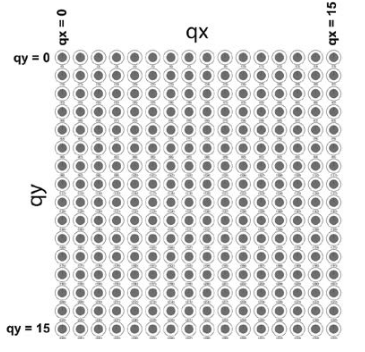
\includegraphics[scale=0.7]{img/holst.png}
	\end{center}
	\captionsetup{justification=centering}
	\caption{Изображение холста в квантовом представлении.}
	\label{img:holst}
\end{figure}

\subsection{Квантовая фаза}

Произвольное квантовое состояние, обозначаемое $\ket{\psi}$, может быть любая суперпозиция, записанная в виде (\ref{for:psi}):
\begin{equation}
	\label{for:psi}
	\ket{\psi} = \alpha\ket{0} + \beta\ket{1}
\end{equation}
 базисных векторов. Согласно условию (\ref{for:ver}) и основываясь на том факте, что глобальная фаза не наблюдаема (то есть $\ket{\psi}$ тоже самое что и $e^{j\gamma}\ket{\psi}$) \cite{global-phase}, выражение (\ref{for:psi}) можно переписать в виде (\ref{for:new_ver}):
 
\begin{equation} 
	\label{for:new_ver}
	\ket{\psi} = \sqrt{1 - p}\ket{0} + e^{j\gamma}\sqrt{p}\ket{1}
\end{equation} где $0 \leq p \leq 1$ -- вероятность того, что бит находится в состоянии 1 и $0 \leq \psi < 2\pi$ -- квантовая фаза (англ. quantum phase).

Применив операцию смены фазы на противоположную (то есть повернуть кубит на 180 градусов), можно изменить состояние кубита аналогично на противоположное. Операцию смены фазы можно применять сразу на несколько кубитов. Таким образом, всего за одну операцию, можно, например, изменить цвет половины (или сразу всех) пикселей синтезируемого изображения. Выигрыш во времени по сравнению с обычными вычислениями очевиден. Используя квантовую фазу можно изображать прямые в квантовом представлении. Пример использования квантовой фазы представлен на рисунке \ref{img:holst_02}.

\begin{figure}[h]
	\begin{center}
		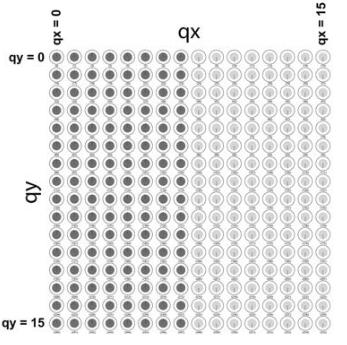
\includegraphics[scale=0.7]{img/holst_02.png}
	\end{center}
	\captionsetup{justification=centering}
	\caption{Переключение фазы для половины изображения.}
	\label{img:holst_02}
\end{figure}

\subsection{Усиление комплексной амплитуды}\label{yka}

Допустим, что у нас имеется четырехкубитный квантовый регистр, который содержит одно из трех квантовых состояний, но мы не знаем какое именно. В каждом из этих состояний присутствует некоторое значение с инвертированной фазой. Назовем его помеченным значением. При чтении из квантового регистра, мы получим случайно число с равномерным распределением, и ничего не сможем узнать о том, какое из трех квантовых состояний было исходным.

Введем зеркальную операцию. Это операция выполняет следующие действия: берёт регистр, находящийся в состоянии $\ket{0}$ и помечает одно из значений регистра с помощью операции смены фазы на противоположную. Теперь амплитуды в каждом состоянии очень сильно различаются, благодаря чему выполнение операции чтения из регистра с большой вероятностью покажет, у какого значения инвертирована фаза -- а следовательно, в каком из состояний находился регистр изначально.

Применении зеркальной операции повторно вернет кубит в исходное состояние. Но, допустим, что при перед повторным использованием так же будет повторна применена операция смены фазы. В результате получится еще одна разность фазы, а вероятность успешного обнаружения помеченного значения возрастает \cite{global-phase}. 

Две эти операции образуют мощную комбинацию. Применяя их вместе, можно увеличивать шанс правильного чтения помеченного значения. Но, к сожалению, бесконечно увеличивая число итераций комбинаций этих операций, невозможно достичь 100\% вероятности правильного чтения значения. В начале итераций, разность амплитуд увеличиваются, и благодаря этому растет вероятность обнаружения правильного значения. Начиная с итерации $N_{AA}$ разность амлпитуд уменьшается, и с каждой итерацией вероятность все ближе становится к исходной, а потом вовсе становится исходной (той, что была без использования итераций \cite{PQC-amplitude}. 

Число $N_{AA}$ можно обозначить как оптимальное количество итераций при усилении комплексной амплитуды. Оно выражается с помощью формулы (\ref{for:optimal}):

\begin{equation}
	\label{for:optimal}
	N_{AA} = \frac{\pi\sqrt{2^{n}}}{4}
\end{equation}

где $n$ -- количество кубитов.


\subsection{Квантовая фазовая логика}

Квантовая фазовая логика инвертирует фазу каждого входного значения, которое дает 1 в результате.
Фазовая логика принципиально отличается от любой традиционной логики -- результаты логических операций скрыты в фазах и их невозможно прочитать. Но, при этом, инвертируя фазы в суперпозиции, можно пометить несколько решений в одном регистре. Кроме того, при использовании инвертирования и усиления комплексной амплитуды можно создавать результаты, доступные для чтения.

С помощью комбинации усилении амплитуды и операций фазовой логики, можно сохранить значение логической операции в фазе состояния \cite{PQC-logic}. Таким образом, мы можем описывать более сложные фигуры, например кривые.

Окружность задается уравнением вида (\ref{for:circle}):

\begin{equation}
	\label{for:circle}
	x^2 + y^2 = r^2
\end{equation}

Предположим, что мы хотим заполнить все пиксели, находящиеся внутри окружности, то есть пиксели, подходящие под условие (\ref{for:circle2}):

\begin{equation}
	\label{for:circle2}
	x^2 + y^2 < r^2
\end{equation}

Для выполнения этого действия нам потребуются выше описанные регистры $qx$ и $qy$, а так же дополнительные регистр-аккумулятор $qacc$. Дальнейший алгоритм таков:

\begin{itemize}
	\item инициализировать регистры $qx$, $qy$ и $qacc$;
	\item ввести регистры $qx$ и $qy$ в суперпозицию;
	\item добавить в регистр $qacc$ сумму квадратов регистров $qx$ и $qy$;
	\item вычесть из регистра $qacc$ квадрат радиуса описываемой окружности;
	\item инвертировать регистр $qacc$ для всех значащих битов;
	\item восстановить регистр $qacc$.
\end{itemize}

\begin{figure}[h]
	\begin{center}
		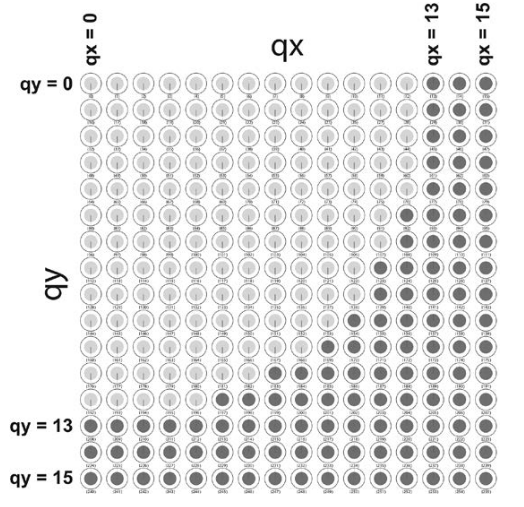
\includegraphics[scale=0.57]{img/holst_03.png}
	\end{center}
	\captionsetup{justification=centering}
	\caption{Переключение кривых на холсте с помощью фазовой логики.}
	\label{for:holst_03}
\end{figure}

\subsection{Квантовое преобразование Фурье}\label{furie}

Квантовое преобразование Фурье позволяет обращаться к скрытой информации, хранящейся в фазах и амплитудах квантового регистра. Данный примитив предоставляет собственный механизм манипуляций с фазами кубитов \cite{PQC-furie}).

Допустим, имеется четырехкубитный квантовый регистр, содержащий одно из трех состояний, но точно неизвестно какое (рисунок \ref{img:furie-example-01}). Как уже говорилось ранее, при чтении регистра будет полученно случайное значение с равномерным распределением. 

\begin{figure}[h]
	\begin{center}
		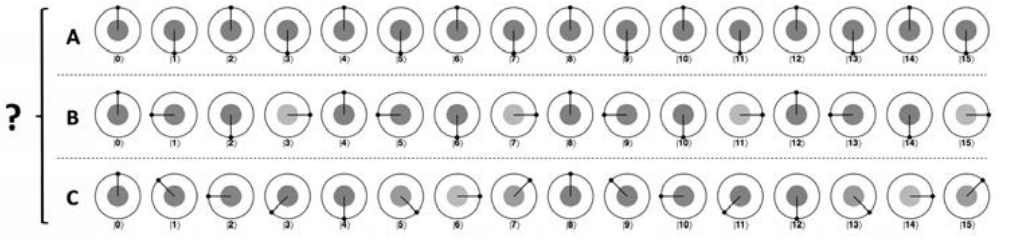
\includegraphics[scale=0.4]{img/furie-example.png}
	\end{center}
	\captionsetup{justification=centering}
	\caption{Три разных состояние кубита до применения квантового преобразования Фурье}
	\label{img:furie-example-01}
\end{figure}

Усиление квантовой амплитуды в данном примере не принесет никакой пользы, так как нет какой-то одной фазы, которая бы выделялась на фоне других в каждом состоянии. Применение квантового преобразования Фурье к рассматриваемому регистру перед чтением результата преобразует каждое из состояний к результату, показанному на рисунке \ref{img:furie-example-02}. Таким образом, можно однозначно определить, какое состояние было исходным.

\begin{figure}[h]
	\begin{center}
		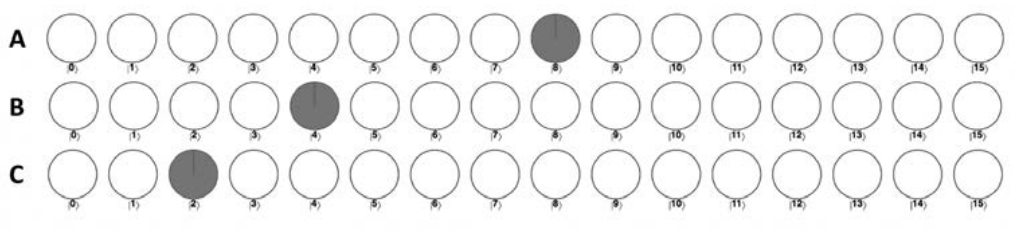
\includegraphics[scale=0.4]{img/furie-example-02.png}
	\end{center}
	\captionsetup{justification=centering}
	\caption{Три разных состояние кубита после применения квантового преобразования Фурье}
	\label{img:furie-example-02}
\end{figure}

Между результатами на рисунке \ref{img:furie-example-01} можно заметить связь: в первом состоянии фаза входного состояния возвращается в 0 восемь раз, а квантовое преобразование Фурье позволяет прочитать значение 8. Во втором состоянии  фаза возвращается к своему начальному состоянию четыре раза, а квантовое преобразование Фурье позволяет прочитать значение 4. Третье состояние подчиняется той же самой закономерности. Квантовое преобразование Фурье успешно открывает частоту сигнала \cite{signal}, содержащуюся в квантовом регистре. Само по себе квантовое преобразование Фурье имеет сильное сходство с классическим механизмом обработки сигналов, называемым дискретным преобразованием Фурье \cite{PQC-furie-proof}.

\section{Квантовая избыточная выборка}

Избыточная выборка -- процесс увеличения число дискретных выборок на пиксель. На один пиксель проецируется не один, а несколько лучей. Результат проекции каждого такого луча сохраняется в соответствующий субпиксель (англ. subpixel). После того, как все нужные выборки сохранены в экранном буфере, итоговый цвет пикселя определяется как усреднённый цвет всех соответствующих ему субпикселей. Таким образом, формула принимает вид (\ref{for:supersampling}): 

\begin{equation}
	\label{for:supersampling}
	res = \frac{sample_{0} + sample_{1} + ... + sample_{n-1}}{n} = \frac{\sum_{i=0}^{n - 1} sample_{i}}{n}
\end{equation}

где:

\begin{itemize}
	\item $res$ -- итоговый цвет пикселя;
	\item $n$ -- количество выборок на пиксель;
	\item $sample_{i}$ -- цвет $i$-ой выборки.
\end{itemize}

В случае квантовой избыточной выборки, для каждого блока необходимо оценить количество субпикселов с инвертированной фазой. Для черных и белых субпикселов (представленных инвертированной или не инвертированной фазой) это позволит нам получить значение для каждого результирующего пиксела, характеризующее интенсивность исходных составляющих субпикселов.

Преимущества использования квантовой избыточной выборки (по сравнению с обычной) связано не с количеством операций графического вывода, а с различиями в характере наблюдаемого шума. В среднем, при сравнении двух идентичных синтезируемых изображения, погрешность на пиксель у квантовой избыточной выборки на 33\% ниже, чем у метода Монте-Карло (обычная избыточная выборка) \cite{PQC-prcnt}. Помимо этого, количество пикселов с нулевой погрешность в среднем в два раза больше, чем у метода Монте-Карло \cite{PQC-prcnt}.

\subsection{Принцип работы}

Основополагающая идея квантовой избыточной выборки заключается в применении метода объединения итераций усиления комплексной амплитуды (\ref{yka}) с квантовым преобразованием Фурье (\ref{furie}). Квантовое преобразование Фурье позволит оценить количество элементов, инвертированных квантовой логикой, используемой в подсхеме инвертирования каждой итерации усиления комплексной амплитуды. В данном случае подсхемой инвертирования является программа, которая инвертирует фазу белых субпикселей.

Определим квантовый регистр, который будет выполнять роль <<счётчика>>. Значение этого регистра будет определять, сколько итераций выполнит наша схема. Введя регистр в суперпозицию, будет выполнено суперпозиция разного количества итераций усиления комплексной амплитуды. Как уже было написано выше, вероятность чтения нескольких инвертированных значений в регистре зависит от количества выполняемых итераций. Кроме этого, колебания вводятся в зависимости от количества инвертированных значений. Таким образом, при выполнении суперпозиции разного количества итераций усиления комплексной амплитуды, вводятся периодические колебания по комплексным амплитудам квантового регистра с частотой, зависящей от количества инвертированных значений.

Для чтения частот, закодированных в квантовых регистра, можно использовать квантовое преобразование Фурье \cite{PQC-fourier}. Зная количество субпикселей, использованных в квантовой выборке, можно определить яркость анализируемого пикселя.

Качество выборки напрямую зависит от количества кубитов для <<счётчиков>>. С увеличением количества образцов (кубитов) вероятность получения точного ответа растёт \cite{PQC-qbits}.

\subsection{Поисковая таблица}\label{table-q}

При запуске квантового алгоритма избыточной выборки и в конце его выполнения читая значение квантового регистра, мы получаем число -- оно связано с количеством белый субпикселей в заданном блоке, но не будет точно равно ему. 

Поисковая таблица квантовой выборки (англ. quantum supersamping lookup table) -- инструмент для определения количества субпикселей в блоке, подразумеваемого считанным значением из квантового регистра. Например, поисковая таблица, для квантовой выборки с размером квантового шейдера $4x4$ и регистром счетчиком, состоящим из четырех кубитов, будет выглядить как таблица с $2^4 = 16$ столбцами и $2^4 = 16$ строками. В строках поисковой таблицы перечисляются возможные результаты чтения значения из квантового регистра. В столбцах перечисляются возможные количества  субпикселей в квантовом шейдере, которые могут привести к такому значению, который был получен путём чтения квантового регистра.

При получении значения из квантового регистра, в поисковой таблице выбирается строка соответствующая считанному значению. Далее, оценивая количество <<белых>> субпикселей, расположенные в этой строке (а точнее лишь вероятность нахождения этих субпикселей в анализируемом пикселе), выбирается конечная яркость пикселя. Из-за того что в строчках расположенны лишь вероятности, появляется некоторая погрешность и не всегда можно  однозначно определить яркость пикселя.

Таким образом, можно описать функцию, на вход принимающую номер строки ($k$) таблицы, и возвращающую вероятность яркости пикселя (\ref{for:table_function}):

\begin{equation}
	\label{for:table_function}
	\gamma(k) = \sum_{i=0}^{n - 1} x_{k_i}
\end{equation}


Поисковая таблица -- характерный признак алгоритма квантовой избыточной выборки. С увеличением размера квантового шейдера (следовательно увеличения количества субпикселей), растёт вероятность точного определения яркости выбранного пикселя.

\begin{figure}[H]
	\begin{center}
		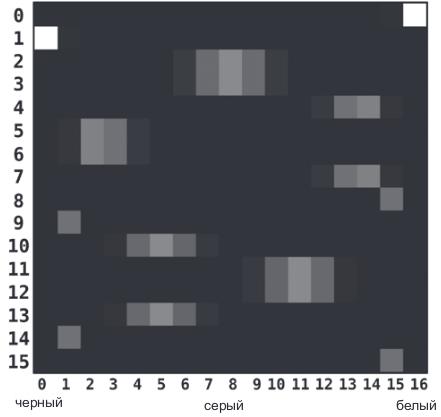
\includegraphics[scale=0.55]{img/qss_table.png}
	\end{center}
	\captionsetup{justification=centering}
	\caption{Поисковая таблица квантовой выборки. По оси OY -- результат квантовой выборки, по оси OX -- цвет пикселя (сумма белых пикселей)}
	\label{img:qss_table}
\end{figure}

\subsection{Карта достоверности}\label{map}

Поисковая таблица также может использоваться для получения вероятности того, что итоговая яркости пиксела выбрана правильно. По расположению считанного значения из квантового регистра, в строке таблицы можно оценить вероятность того, что полученное значение было правильным. Для каждого значения из выбранной строки имеется вероятность что данный субпиксель является белым -- это можно сделать с помощью расположения считанного значения (в процессе избыточной выборки) в соответствующей строке таблице поиска. По этим результатам можно построить <<карту достоверности>> (англ. confidence map), обозначающую вероятное расположение ошибок в синтезируемом изображении.

\begin{figure}[H]
	\begin{center}
		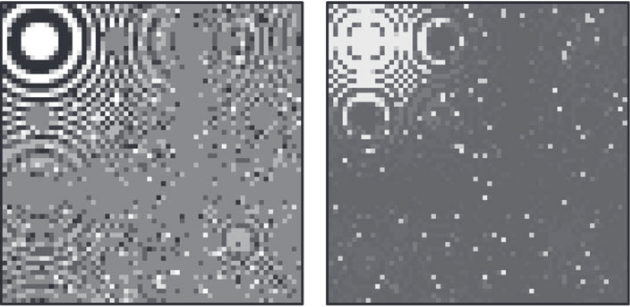
\includegraphics[scale=0.6]{img/map.png}
	\end{center}
	\captionsetup{justification=centering}
	\caption{Карта достоверности. Слева -- результат квантовой выборки, справа -- карта достоверности на уровне пикселей.}
	\label{img:map}
\end{figure}

\section{Колоризация изображения}

Фазы и комплексные амплитуды квантового регистра можно использовать для кодирования более широкого диапазона цветовых значений (помимо белого и черного), но тогда метод квантовой избыточной выборки работать не будет \cite{PQC-color}. 

Для колоризации изображения можно воспользоваться технологией битовых слоёв. Квантовый пиксельный шейдер будет использоваться для построения отдельных монохромных изображений, каждое из которых будет представлять один бит изображения. Таким образом, пиксельный шейдер фактически будет генерировать $N$ монохромных изображений, где $N$ -- количество цветов, которые нужно <<запутать>> в изображении. Все эти $N$ изображений пройдут квантовую избыточную выборку по отдельности и будут объединены в итоговое цветное изображение.

\section*{Вывод}

В данном разделе был проведен анализ квантовых алгоритмов и структур данных, которые возможно использовать в поставленной задаче. В качестве ключевого алгоритма, который может улучшить качество синтезируемого изображения, выбран алгоритм квантовой избыточной выборки, в сочетании с такими структурами данных как квантовая поисковая таблица и квантовая карта достоверности. Именно этот алгоритм и будет реализован в рамках данной работы.